\chapter{Computing}\label{ch:intro}
\slatexignorecurrentfile

\chapquote{In their capacity as a tool, computers will be but a ripple on the surface of our culture. In their capacity as intellectual challenge, they are without precedent in the cultural history of mankind.}{Edsger Dijkstra, 1972 Turing Award Lecture}

\topics{}

%\margintag{Tools amplify and extend abilities}
The first million years of hominid history produced tools to amplify, and later mechanize, our physical abilities to enable us to move faster, reach higher, and hit harder.  We have developed tools that amplify physical force by the trillions and increase the speeds at which we can travel by the thousands.  

Tools that amplify intellectual abilities are much rarer.  While some animals have developed tools to amplify their physical abilities, only humans have developed tools to substantially amplify our intellectual abilities and it is those advances that have enabled humans to dominate the planet.  The first key intellect amplifier was language.  Language provided the ability to transmit our thoughts to others, as well as to use our own minds more effectively.  The next key intellect amplifier was writing, which enabled the storage and transmission of thoughts over time and distance.  %This book focuses on the most recent major mental amplifier and extender: {\em computing}.  

%In a strong sense, 
Computing is the ultimate mental amplifier---\cut{other than practical limits on space and time, }computers can mechanize any intellectual activity we can imagine.  Automatic computing radically changes how humans solve problems, and even the kinds of problems we can imagine solving.  Computing has changed the world more than any other invention of the past hundred years, and has come to pervade nearly all human endeavors.  Yet, we are just at the beginning of the computing revolution; today's computing offers just a glimpse of the potential impact of computing.   

There are two reasons why everyone should study computing:
\marginquote{It may be true that you have to be able to read in order to fill out forms at the DMV, but that's not why we teach children to read. We teach them to read for the higher purpose of allowing them access to beautiful and meaningful ideas.}{Paul Lockhart\index{people}{Lockhart, Paul}, {\em Lockhart's~Lament}}
\begin{enumtight}
\item Nearly all of the most exciting and important technologies, arts, and sciences of today and tomorrow are driven by computing.
\item Understanding computing illuminates deep insights and questions into the nature of our minds, our culture, and our universe.
\end{enumtight}

Anyone who has submitted a query to Google\cut{\index{general}{Google}}, watched \emph{Toy Story}\cut{\index{general}{Toy Story}}, had LASIK eye surgery, used a smartphone, seen a Cirque Du Soleil show, shopped with a credit card, or microwaved a pizza\cut{\index{general}{pizza}} should be convinced of the first reason.  None of these would be possible without the tremendous advances in computing over the past half century. 

Although this book will touch on on some exciting applications of computing, our primary focus is on the second reason, which may seem more surprising.  Computing changes how we think about problems and how we understand the world.  The goal of this book is to teach you that new way of thinking.

\section{Processes, Procedures, and Computers}\label{sec:processes}

Computer science is the study of \definition{information processes}.  A process is a sequence of steps.  Each step changes the state of the world in some small way, and the result of all the steps produces some goal state. For example, baking a cake, mailing a letter, and planting a tree are all processes.  Because they involve physical things like sugar and dirt, however, they are not pure information processes.  Computer science focuses on processes that involve abstract information rather than physical things.  


The boundaries between the physical world and pure information processes, however, are often fuzzy.  Real computers operate in the physical world: they obtain input through physical means (e.g., a user pressing a key on a keyboard that produces an electrical impulse), and produce physical outputs (e.g., an image displayed on a screen).  By focusing on abstract information, instead of the physical ways of representing and manipulating information, we simplify computation to its essence to better enable understanding and reasoning.

%\footnote{This is actually a subtle point.  Most computing processes do eventually result in physical outcomes such as displaying an image on a screen or adjusting the pressure on an anti-lock brake
%Ultimately, information \emph{is} represented by physical things, and physical things contain information.  For the first [several] chapters, we consider information abstractly; we'll get into some of the complexities of physical representation of information [later?]}.

A \definition{procedure} is a description of a process.  A simple process can be described just by listing the steps.  The list of steps is the procedure; the act of following them is the process.  A procedure that can be followed without any thought is called a \emph{mechanical procedure}.  An \definition{algorithm} is a mechanical procedure that is guaranteed to eventually finish.

For example, here is a procedure for making coffee\index{general}{coffee}, adapted from the actual directions that come with a major coffeemaker: \marginquote{A mathematician is a machine for turning coffee into theorems.}{Attributed to Paul Erd\"{o}s\index{people}{Erd\"{o}s, Paul}}
\begin{enumtight}
\item Lift and open the coffeemaker lid.
\item Place a basket-type filter into the filter basket.
\item Add the desired amount of coffee and \cut{gently }shake to level the coffee.
\item Fill the decanter with cold, fresh water to the desired capacity.
\item Pour the water into the water reservoir.
\item Close the lid.
\item Place the empty decanter on the warming plate.
\item Press the ON button.
\end{enumtight}

Describing processes by just listing steps like this has many limitations.  First, natural languages are very imprecise and ambiguous.  Following the steps correctly requires knowing lots of unstated assumptions.  For example, step three assumes the operator understands the difference between coffee grounds and finished coffee, and can infer that this use of ``coffee'' refers to coffee grounds since the end goal of this process is to make drinkable coffee.  Other steps assume the coffeemaker is plugged in and sitting on a flat surface. \cut{\marginquote{I have no idea what you're talking about when you say~``ask''.}{Bill Gates, deposition in Microsoft anti-trust trial}} 

One could, of course, add lots more details to our procedure and make the language more precise than this.  Even when a lot of effort is put into writing precisely and clearly, however, natural languages such as English are inherently ambiguous. This is why the United States tax code is 3.4 million words long, but lawyers can still spend years arguing over what it really means. 

Another problem with this way of describing a procedure is that the size of the description is proportional to the number of steps in the process.  This is fine for simple processes that can be executed by humans in a reasonable amount of time, but the processes we want to execute on computers involve trillions of steps.  This means we need more efficient ways to describe them than just listing each step one-by-one.  \cut{The languages we use to program computers provide ways to define long and complex processes with short procedures.}

\begin{comment}
People have been developing procedures for thousands of years.  For example, in \emph{Elements} (300 BC), Euclid describes a procedure for computing the greatest common divisor of two numbers.  The full procedure is not important to understand here, but what is relevant is how he described it:
\begin{quote}
Let AB and CD be the two given numbers not relatively prime. It is required to find the greatest common divisor of AB and CD.

If now CD divides AB, since it also divides itself, then CD is a common measure of CD and AB. And it is manifest that it is also the greatest, for no greater number than CD divides CD. 

But, if CD does not measure AB, then, when the less of the numbers AB and CD being continually subtracted from the greater, some number is left which measures the one before it.

For a unit is not left, otherwise AB and CD would be relatively prime, which is contrary to the hypothesis.

Therefore some number is left which measures the one before it.

...

If CF is not the greatest common measure of AB and CD, then some number G, which is greater than CF, measures the numbers AB and CD.

\end{quote}
\end{comment}

To program computers, we need tools that allow us to describe processes precisely and succinctly.  Since the procedures are carried out by a machine, every step needs to be described; we cannot rely on the operator having ``common sense'' (for example, to know how to fill the coffeemaker with water without explaining that water comes from a faucet, and how to turn the faucet on).  Instead, we need mechanical procedures that can be followed without any thinking.

A \definition{computer} is a machine that can:
\begin{enumtight}
\item Accept input.  Input could be entered by a human typing at a keyboard, received over a network, or provided automatically by sensors attached to the computer.
\item Execute a mechanical procedure, that is, a procedure where each step can be executed without any thought.
\item Produce output.  Output could be data displayed to a human, but it could also be anything that effects the world outside the computer such as electrical signals that control how a device operates.
\end{enumtight}

\marginquote{A computer terminal is not some clunky old television with a typewriter in front of it. It is an interface where the mind and body can connect with the universe and move bits of it about.}{Douglas Adams}
Computers exist in a wide range of forms, and thousands of computers are hidden in devices we use everyday but don't think of as computers such as cars, phones, TVs, microwave ovens, and access cards.  \LATER{In the next chapter, we provide a more formal definition of a computer and provide some examples of simple mechanical ways to perform computation.}  Our primary focus is on \emph{universal computers}, which are computers that can perform {\em all} possible mechanical computations on discrete inputs except for practical limits on space and time.  The next section explains what it discrete inputs means; Chapters~\ref{ch:machines} and~\ref{ch:computability} explore more deeply what it means for a computer to be universal.
%\profile{Ada, Countess of Lovelace}{}

\section{Measuring Computing Power}\label{sec:computing-power}

For physical machines, we can compare the power of different machines by measuring the amount of mechanical work they can perform within a given amount of time.  This power can be captured with units like {\em horsepower} and {\em watt}.  Physical power is not a very useful measure of computing power, though, since the amount of computing achieved for the same amount of energy varies greatly\LATER{(see Exercise~\ref{ex:power})}.  Energy is consumed when a computer operates, but consuming energy is not the purpose of using a computer.

Two properties that measure the power of a computing machine are:
\begin{enumtight}
\item {\em How much information} it can process?  
%Note that the information it processes includes the program as well as the input data to that program and any space needed to keep track of intermediate results.
\item {\em How fast} can it process?  
%For a given program and input, how long does it take before the process completes with the result?
\end{enumtight}

We defer considering the second property until Part II, but consider the first question here.  

\subsection{Information}\label{sec:information}

Informally, we use \definition{information} to mean knowledge.  But to understand information quantitatively, as something we can measure, we need a more precise way to think about information.  

The way computer scientists measure information is based on how what is known changes as a result of obtaining the information.  The primary unit of information is a \definition{bit}.  {\em One bit} of information {\em halves} the amount of uncertainty.  It is equivalent to answering a ``yes'' or ``no'' question, where either answer is equally likely beforehand.  Before learning the answer, there were two possibilities; after learning the answer, there is one.  

We call a question with two possible answers a \definition{binary question}.  Since a bit can have two possible values, we often represent the values as {\bf 0} and \bit{1}.

For example, suppose we perform a fair coin toss but do not reveal the result.  Half of the time, the coin will land ``heads'', and the other half of the time the coin will land ``tails''.  Without knowing any more information, our chances of guessing the correct answer are $\frac{1}{2}$.  One bit of information would be enough to convey either ``heads'' or ``tails''; we can use {\bf 0} to represent ``heads'' and \bit{1} to represent ``tails''.  So, the amount of information in a coin toss is one bit.  

Similarly, one bit can distinguish between the values 0 and 1:

\begin{center}
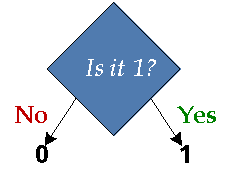
\includegraphics[height=1.0in]{figures/onebit.pdf} 
\end{center}

\begin{example}{Dice} How many bits of information are there in the outcome of tossing a six-sided die?

There are six equally likely possible outcomes, so without any more information we have a one in six chance of guessing the correct value.  One bit is not enough to identify the actual number, since one bit can only distinguish between two values.  We could use five binary questions like this:

\begin{center}
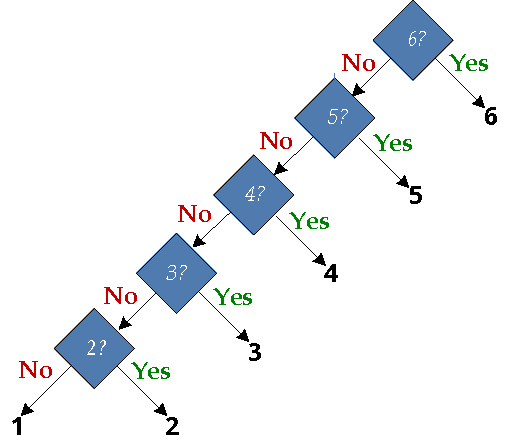
\includegraphics[width=2.5in]{figures/sixchoices.pdf} 
\end{center}

This is quite inefficient, though, since we need up to five questions to identify the value (and on average, expect to need $3\frac{1}{3}$ questions).  Can we identify the value with fewer than 5 questions?

Our goal is to identify questions where the ``yes'' and ``no'' answers are equally likely---that way, each answer provides the most information possible.  This is not the case if we start with, ``Is the value 6?'', since that answer is expected to be ``yes'' only one time in six.  Instead, we should start with a question like, ``Is the value at least 4?''.  Here, we expect the answer to be ``yes'' one half of the time, and the ``yes'' and ``no'' answers are equally likely.  If the answer is ``yes'', we know the result is 4, 5, or 6.  With two more bits, we can distinguish between these three values (note that two bits is actually enough to distinguish among {\em four} different values, so some information is wasted here).  Similarly, if the answer to the first question is no, we know the result is 1, 2, or 3.  We need two more bits to distinguish which of the three values it is.  Thus, with three bits, we can distinguish all six possible outcomes.  

\begin{center}
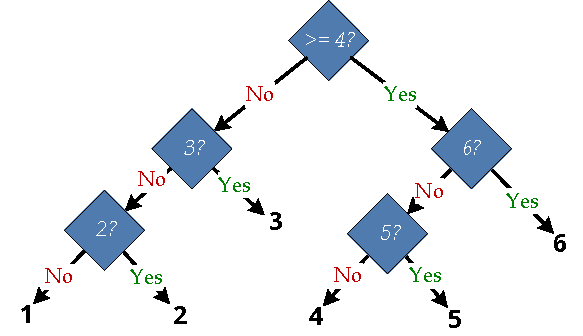
\includegraphics[width=3.7in]{figures/sixchoices-better.pdf}
\end{center}

Three bits can convey more information that just six possible outcomes, however.  In the binary question tree, there are some questions where the answer is not equally likely to be ``yes'' and ``no'' (for example, we expect the answer to ``Is the value 3?'' to be ``yes'' only one out of three times).  Hence, we are not obtaining a full bit of information with each question.  

Each bit doubles the number of possibilities we can distinguish, so with three bits we can distinguish between $2 * 2 * 2 = 8$ possibilities.  In general, with $n$ bits, we can distinguish between $2^n$ possibilities.  Conversely, distinguishing among $k$ possible values requires $\log_2 k$ bits.  The \definition{logarithm} is defined such that if $a=b^c$ then $\log_b a = c$.  Since each bit has two possibilities, we use the logarithm base 2 to determine the number of bits needed to distinguish among a set of distinct possibilities.
For our six-sided die, $\log_2 6 \approx 2.58$, so we need approximately 2.58 binary questions.  But, questions are discrete: we can't ask $0.58$ of a question, so we need to use three binary questions.
\end{example}

\shortsection{Trees} Figure~\ref{fig:three-bits} depicts a structure of binary questions for distinguishing among eight values.  We call this structure a \definition{binary tree}.  We will see many useful applications of tree-like structures in this book.  

Computer scientists draw trees upside down.  The \emph{root} is the top of the tree, and the \emph{leaves} are the numbers at the bottom (\snumber{0}, \snumber{1}, \snumber{2}, $\ldots$, \snumber{7}).  There is a unique path from the root of the tree to each leaf.  Thus, we can describe each of the eight possible values using the answers to the questions down the tree.  For example, if the answers are ``No'', ``No'', and ``No'', we reach the leaf \snumber{0}; if the answers are ``Yes'', ``No'', ``Yes'', we reach the leaf \snumber{5}.  Since there are no more than two possible answers for each node, we call this a \emph{binary} tree.

We can describe any non-negative integer using bits in this way, by just adding additional levels to the tree.  For example, if we wanted to distinguish between 16 possible numbers, we would add a new question, ``Is is $>=$ 8?'' to the top of the tree.  If the answer is ``No'', we use the tree in Figure~\ref{fig:three-bits} to distinguish numbers between 0 and 7.  If the answer is ``Yes'', we use a tree similar to the one in Figure~\ref{fig:three-bits}, but add 8 to each of the numbers in the questions and the leaves.  

The \definition{depth} of a tree is the length of the longest path from the root to any leaf.  The example tree has depth three.  A binary tree of depth $d$ can distinguish up to $2^d$ different values.

\begin{figure}[th]
\begin{center}
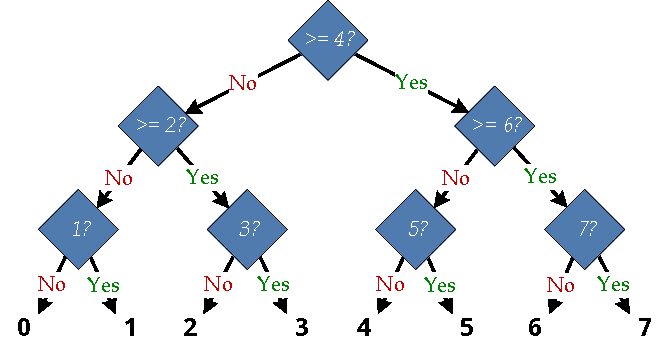
\includegraphics[width=4.5in]{figures/three-bits.pdf}
\end{center}
\caption{Using three bits to distinguish eight possible values.}\label{fig:three-bits}
\end{figure}

\shortsection{Units of Information}  One \emph{byte} is defined as eight bits.  Hence, one byte of information corresponds to eight binary questions, and can distinguish among $2^8$ (256) different values.  For larger amounts of information, we use metric prefixes, but instead of scaling by factors of 1000 they scale by factors of $2^{10}$ (1024).  Hence, one \emph{kilobyte} is 1024 bytes; one \emph{megabyte} is $2^{20}$ (approximately one million) bytes; one \emph{gigabyte} is $2^{30}$ (approximately one billion) bytes; and one \emph{terabyte} is $2^{40}$  (approximately one trillion) bytes.

\beforeex
\begin{exercise}
Draw a binary tree with the minimum possible depth to:
\begin{subexerciselist}
\item Distinguish among the numbers $0, 1, 2, \ldots, 15$.

\solution{
There are sixteen ($2^4$) different numbers, so the minimum depth binary tree has four levels.  There are many different trees that could work, so long as each decision divides the remaining possible numbers in two equal-sized sets.  The easiest way to construct it is to start with the 3-bit tree in Figure~\ref{fig:three-bits} which distinguishes 0--7.  We make two copies of this, but add $8$ to each number in the second copy, and add an extra binary question at the top to decide which subtree to use.

\begin{center}
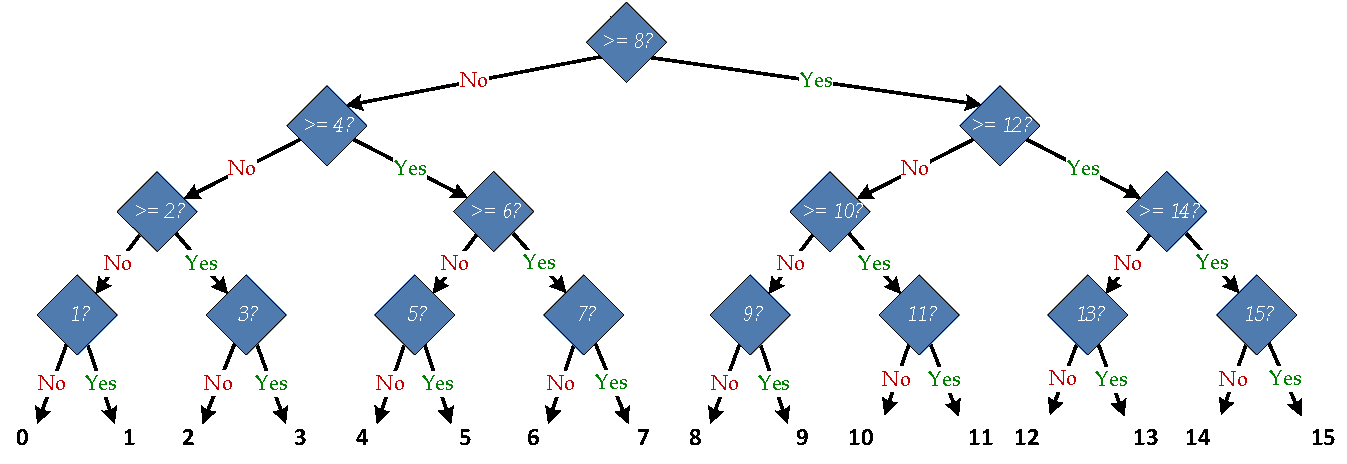
\includegraphics[width=4.8in]{figures/exercise-fourbits.pdf}
\end{center}
}

\item Distinguish among the 12 months of the year.

\solution{Since there are 12 months, we need $\log_2 12 \approx 3.58$ bits to distinguish them.  This means we need a tree with 4 levels, but on some paths only three questions are needed. One solution would be to use 0--11 from the previous solution.  A more natural solution might divide the year into quarters.

\begin{center}
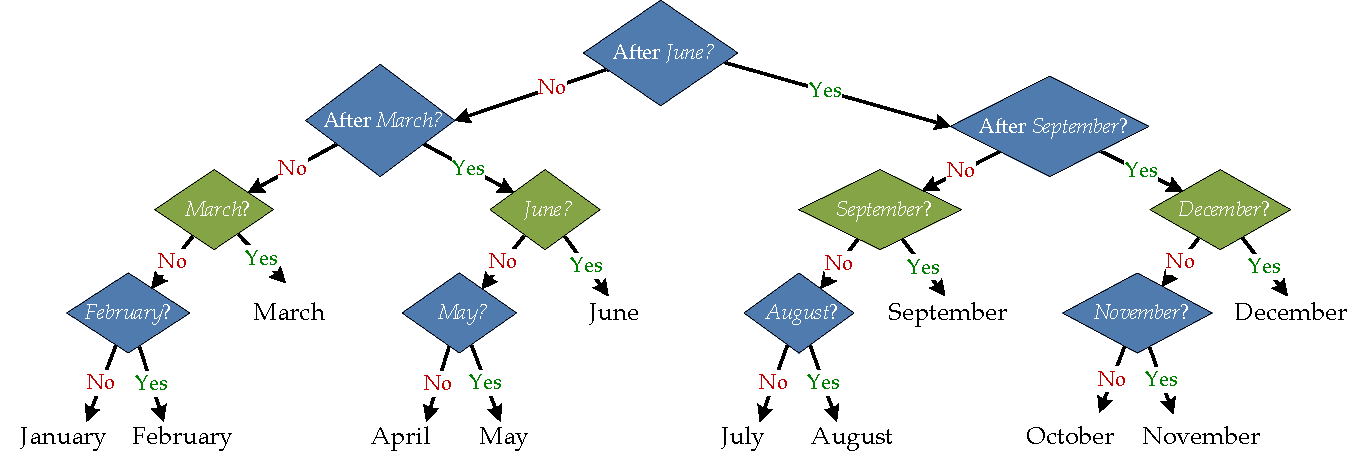
\includegraphics[width=4.6in]{figures/exercise-months.pdf}
\end{center}

Note that the answers for the green boxes do not provide a full bit of information since the ``No'' answer leads to two leaf nodes (e.g., January and February), but the ``Yes'' answer only leads to one leaf node (e.g., March).  If each month is equally likely, the answer should be ``No'' two thirds of the time.
}


\end{subexerciselist}
\end{exercise}
\afterex

\beforeex
\begin{exercise}
How many bits are needed: 
\begin{subexerciselist}
\item To uniquely identify any currently living human? 

\solution{
According to the U. S. Census Bureau, the world population (on July 4, 2011) is 6.95 Billion people.  See \url{http://www.census.gov/main/www/popclock.html} for an updated count.  To identify each person, we need $$\lceil{\log_2 6,950,000,000}\rceil = 33 \textrm{ bits}$$ 
(the notation $\lceil x \rceil$ means the ``ceiling'' of $x$ which is the least integer larger than $x$)k.  Since $2^33 = 8,589,934,592$, 33 bits should be enough to uniquely identify every living person for at least the next decade.}  

\item To uniquely identify any human who ever lived? 

\solution{
This is much tougher, and requires defining a \emph{human}.  The best estimate I can find come from Carl Haub's article for the Population Reference Bureau, originally written in 1995 and updated in 2002 (\url{http://www.prb.org/Articles/2002/HowManyPeopleHaveEverLivedonEarth.aspx}).  He estimated that modern humans emerged about 50,000 years ago, and that the total number of humans born up to 2002 was 106 Billion.  The world birth rate is approximately 130 million per year, so a current estimate would be perhaps 1-2 Billion more.  So, 36 bits is certainly not enough ($2^36 = 68,719,476,736$), but 37 bits should be enough for a long time ($2^37 = 137,438,953,472$).
}

\item To identify any location on Earth within one square centimeter? 
\solution{
The total surface area of the Earth is $510,072,000 \textrm{km}^2$.  One kilometer is $100*1000 = 100,000$ centimeters, so one square kilometer is $(100*1000)^2 = 10,000,000,000$ square centimeters.  So, the total surface area of the Earth is 
$5,100,720,000,000,000,000$ square centimeters.  The number of bits needed to represent this is $\log_2 5,100,720,000,000,000,000 \approx 62.145$ so $63$ bits is enough to uniquely identify every square centimeter of the Earth's surface.  (For comparison, Internet addresses are $128$ bits.  This is enough for each square centimeter of the Earth to have 
over 66 quadrillion IP addresses!)  
}

\item To uniquely identify any atom in the observable universe?
\solution{
The number of atoms in the universe is estimated to be $10^{80}$ (see \url{http://en.wikipedia.org/wiki/Observable_universe} for a good explanation of how this number was derived).  To determine the number of bits needed to uniquely identify every atom, we need to convert from decimal to binary.  It requires $\log_2 10 \approx 3.32$ bits to represent each decimal digit, so $10^{80} \approx 2^{265.7}$.  Hence, $266$ bits is enough to uniquely identify every atom in the universe.
}

\end{subexerciselist}
\end{exercise}
\afterex

\beforesplitex
\begin{exercise}
The examples all use binary questions for which there are two possible answers.  Suppose instead of basing our decisions on bits, we based it on \emph{trits} where one trit can distinguish between three equally likely values.  For each trit, we can ask a ternary question (a question with three possible answers).
\begin{subexerciselist}
\item \greenstar How many trits are needed to distinguish among eight possible values?  (A convincing answer would show a ternary tree with the questions and answers for each node, and argue why it is not possible to distinguish all the values with a tree of lesser depth.)

\solution{
Two trits are required since $log_3 8 \approx 1.893$.  Here is one such tree:
\begin{center}
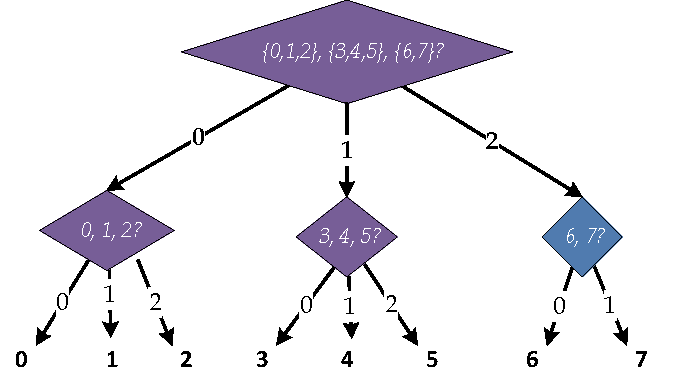
\includegraphics[width=4.0in]{figures/exercise-trits.pdf}
\end{center}
All of the decision nodes except for the bottom rightmost one use three possible outputs.  Hence, we could distinguish one additional value using 2 trits (which makes sense since $3^2 = 9$).
}

\item \goldstar Devise a general formula for converting between bits and trits.  How many trits does it require to describe $b$ bits of information?
\solution{
To convert between logarithm bases, we use the formula 
$$
\log_b x = \frac{\log_a x}{\log_a b}.
$$
So, for a $n$-bit value $x$,
$$
\log_3 x = \frac{n}{log_2 3} \approx 0.63093 n
$$
Thus, to represent an $n$-bit value requires up to $\lceil 0.63093 n \rceil$ trits.
}
\end{subexerciselist}
\end{exercise}
\aftersplitex

\splitexplorenobar{Guessing Numbers}{The guess-a-number game starts with one player (the \emph{chooser}) picking a number between 1 and 100 (inclusive) and secretly writing it down.  The other player (the \emph{guesser}) attempts to guess the number.  After each guess, the chooser responds with ``correct'' (the guesser guessed the number and the game is over), ``higher'' (the actual number is higher than the guess), or ``lower'' (the actual number is lower than the guess).  
\begin{subexerciselist}
\item Explain why the guesser can receive slightly more than one bit of information for each response.
\item Assuming the chooser picks the number randomly (that is, all values between 1 and 100 are equally likely), what are the best first guesses?  Explain why these guesses are better than any other guess.  (Hint: there are two equally good first guesses.)
\item \bluestar What is the maximum number of guesses the second player should need to always find the number?
\item \greenstar What is the average number of guesses needed (assuming the chooser picks the number randomly as before)?
\item \goldstar Suppose instead of picking randomly, the chooser picks the number with the goal of maximizing the number of guesses the second player will need.  What number should she pick?  
\item \doublegoldstar How should the guesser adjust her strategy if she knows the chooser is picking adversarially?
\item \doublegoldstar What are the best strategies for both players in the adversarial guess-a-number game where chooser's goal is to pick a starting number that maximizes the number of guesses the guesser needs, and the guesser's goal is to guess the number using as few guesses as possible.
\end{subexerciselist}
}

\splitexplore{Twenty Questions}{The two-player game \emph{twenty questions} starts with the first player (the \emph{answerer}) thinking of an object, and declaring if the object is an animal, vegetable, or mineral (meant to include all non-living things).  
After this, the second player (the \emph{questioner}), asks binary questions to try and guess the object the first player thought of.  The first player answers each question ``yes'' or ``no''.  
The website \url{http://www.20q.net/} offers a web-based twenty questions game where a human acts as the answerer and the computer as the questioner.  The game is also sold as a \$10 stand-alone toy (shown in the picture).  
\sidepicture{0.18}{images/20q_original.jpg}{20Q Game}{Image from ThinkGeek} %http://www.thinkgeek.com/images/products/zoom/20q_original.jpg
\begin{subexerciselist}
\item How many different objects can be distinguished by a perfect questioner for the standard twenty questions game?
\item What does it mean for the questioner to play perfectly?
\item Try playing the 20Q game at \url{http://www.20q.net}.  Did it guess your item?
\item Instead of just ``yes'' and ``no'', the 20Q game offers four different answers: ``Yes'', ``No'', ``Sometimes'', and ``Unknown''.  (The website version of the game also has ``Probably'', ``Irrelevant'', and ``Doubtful''.)  If all four answers were equally likely (and meaningful), how many items could be distinguished in 20 questions?
\item For an Animal, the first question 20Q sometimes asks is ``Does it jump?'' (20Q randomly selected from a few different first questions).  Is this a good first question?  
\item \goldstar How many items do you think 20Q has data for? 
\item \doublegoldstar Speculate on how 20Q could build up its database.
\end{subexerciselist}
}
%!\sidepicture{0.3}{images/20q_original.jpg}{20Q Game}{Image from ThinkGeek}

\subsection{Representing Data}\label{sec:representingdata}

We can use sequences of bits to represent many kinds of data.  All we need to do is think of the right binary questions for which the bits give answers that allow us to represent each possible value.  Next, we provide examples showing how bits can be used to represent numbers, text, and pictures.

\shortsection{Numbers} In the previous section, we identified a number using a tree where each node asks a binary question and the branches correspond to the ``Yes'' and ``No'' answers.  A more compact way of writing down our decisions following the tree is to use \bit{0} to encode a ``No'' answer, and \bit{1} to encode a ``Yes'' answer and describe a path to a leaf by a sequence of \bit{0}s and \bit{1}s---the ``No'', ``No'', ``No'' path to \bit{0} is encoded as \bits{000}, and the ``Yes'', ``No'', ``Yes'' path to \snumber{5} is encoded as \bits{101}.  This is known as the \indexeddefinition{binary number system}{binary numbers}.  Whereas the decimal number system uses ten as its base (there are ten decimal digits, and the positional values increase as powers of ten), the binary system uses two as its base (there are two binary digits, and the positional values increase as powers of two).\marginquote{There are only 10 types of people in the world: those~who~understand~binary, and~those~who~don't.}{Infamous T-Shirt} 

For example, the binary number \bits{10010110} represents the decimal value \snumber{150}:
%\begin{displaymath}
%0*2^{0} + 1*2^{1} + 1*2^{2} + 0*2^{3} + 1*2^{4} + 0*2^{5} + 0*2^{6} + 1*2^{7} %$= 2 + 4 + 16 + 128 = 150$.
%\end{displaymath}
\begin{center}
\begin{tabular}{|r|c|c|c|c|c|c|c|c|} \hline
Binary: & \bit{1} & \bit{0} & \bit{0} & \bit{1} & \bit{0} & \bit{1} & \bit{1} & \bit{0} \\ \hline 
Value: & $2^7$ & $2^6$ & $2^5$ & $2^4$ & $2^3$ & $2^2$ & $2^1$ & $2^0$ \\ \hline
Decimal Value:& 128 & 64 & 32 & 16 & 8 & 4 & 2 & 1 \\ \hline
\end{tabular}
\end{center}
As in the decimal number system, the value of each binary digit depends on its position.

By using more bits, we can represent larger numbers.  With enough bits, we can represent any natural number this way. The more bits we have, the larger the set of possible numbers we can represent.  
As we saw with the binary decision trees, $n$ bits can be used to represent $2^{n}$ different numbers.  
%Hence, we can use bits to measure the amount of information in a number, but what about the amount of information in a poem or a picture? 

\shortsection{Discrete Values}\index{general}{discrete} We can use a finite sequence of bits to describe {\em any} value that is selected from a \emph{countable} set of possible values.  A set is \definition{countable} if there is a way to assign a unique natural number to each element of the set.  All finite sets are countable.  Some, but not all, infinite sets are countable.  For example, there appear to be more integers than there are natural numbers since for each natural number, $n$, there are two corresponding integers, $n$ and $-n$.  But, the integers are in fact countable.  We can enumerate the integers as: $0, 1, -1, 2, -2, 3, -3, 4, -4, \ldots$ and assign a unique natural number to each integer in turn.  

Other sets, such as the real numbers, are uncountable.  Georg Cantor proved this using a technique known as \definition{diagonalization}.  Suppose the real numbers are enumerable.  This means we could list all the real numbers in order, so we could assign a unique integer to each number.  For example, considering just the real numbers between 0 and 1, our enumeration might be:

\begin{tabular}[c]{rl}
1     & $.\textcolor{blue}{0}0000000000000\ldots$ \\
2     & $.2\textcolor{blue}{5}000000000000\ldots$ \\
3     & $.33\textcolor{blue}{3}33333333333\ldots$ \\
4     & $.666\textcolor{blue}{6}666666666\ldots$ \\
$\cdots$ & $\cdots$ \\
57236 & $.141592653589793\ldots$\\
$\cdots$ & $\cdots$ \\
\end{tabular}

Cantor proved by contradiction that there is no way to enumerate all the real numbers.  The trick is to produce a new real number that is not part of the enumeration.  We can do this by constructing a number whose first digit is different from the first digit of the first number, whose second digit is different from the second digit of the second number, etc.  For the example enumeration above, we might choose $.1468\ldots$.  

The $k^{th}$ digit of the constructed number is different from the $k^{th}$ digit of the number $k$ in the enumeration.  Since the constructed number differs in at least one digit from every enumerated number, it does not match any of the enumerated numbers exactly.  Thus, there is a real number that is not included in the enumeration list, and it is impossible to enumerate all the real numbers.\footnote{Alert readers should be worried that this isn't quite correct since the resulting number may be a different way to represent the same real number (for example, $.1999999999999\ldots = .20000000000\ldots$ even though they differ in each digit).  This technical problem can be fixed by placing some restrictions on how the modified digits are chosen to avoid infinite repetitions.}

Digital computers\footnote{This is, indeed, part of the definition of a digital computer.  An \emph{analog computer} operates on continuous values. In Chapter~\ref{ch:machines}, we explain more of the inner workings of a computer and why nearly all computers today are digital.  We use \emph{computer} to mean a \emph{digital computer} in this book. The property that there are more real numbers than natural numbers has important implications for what can and cannot be computed, which we return to in Chapter~\ref{ch:computability}.} operate on inputs that are discrete values.  Continuous values, such as real numbers, can only be approximated by computers.  Next, we consider how two types of data, text and images, can be represented by computers.  The first type, text, is discrete and can be represented exactly; images are continuous, and can only be represented approximately.

\shortsection{Text} The set of all possible sequences of characters is countable.  One way to see this is to observe that we could give each possible text fragment a unique number, and then use that number to identify the item.  For example we could enumerate all texts alphabetically by length (here, we limit the characters to lowercase letters):
%\begin{quote}
{\sf a}, {\sf b}, {\sf c}, $\ldots$, {\sf z}, {\sf aa}, {\sf ab}, $\ldots$, {\sf az}, {\sf ba}, $\ldots$, {\sf zz}, {\sf aaa}, $\ldots$
%\end{quote}

Since we have seen that we can represent all the natural numbers with a sequence of bits, so once we have the mapping between each item in the set and a unique natural number, we can represent all of the items in the set.  For the representation to be useful, though, we usually need a way to construct the corresponding number for any item directly.

So, instead of enumerating a mapping between all possible character sequences and the natural numbers, we need a process for converting any text to a unique number that represents that text.  Suppose we limit our text to characters in the standard English alphabet.  If we include lower-case letters (26), upper-case letters (26), and punctuation (space, comma, period, newline, semi-colon), we have 57 different symbols to represent.  We can assign a unique number to each symbol, and encode the corresponding number with six bits (this leaves seven values unused since six bits can distinguish 64 values).  For example, we could encode using the mapping shown in Table~\ref{tab:alphabet}.  The first bit answers the question: ``Is it an uppercase letter after {\bf F} or a special character?''.  When the first bit is \bit{0}, the second bit answers the question: ``Is it after {\bf p}?''.

%%\begin{center}
\begin{table}[!ht]\small
\centering
\begin{minipage}[t]{0.3\linewidth}
\centering
\begin{tabular}{|c|c|}\hline
a & \bits{000000} \\
b & \bits{000001} \\
c & \bits{000010} \\
d & \bits{000011} \\
$\cdots$ & $\cdots$ \\
p & \bits{001111} \\
q & \bits{010000} \\
$\cdots$ & $\cdots$ \\
z & \bits{011001} \\ \hline
\end{tabular}
\end{minipage}
\hspace{0.15cm}
\begin{minipage}[t]{0.3\linewidth}
\centering
\begin{tabular}{|c|c|}\hline
A & \bits{011010} \\
B & \bits{011011} \\
C & \bits{011100} \\
$\cdots$ & $\cdots$ \\
F & \bits{011111} \\ 
G & \bits{100000} \\
$\cdots$ & $\cdots$ \\
% I 100010
% J 100011
% K 100100
% L 100101
% M 100110
% N 100111
% O 101000
% P 101001
% Q 101010
% R 101011
% S 101100
% T 101101
% U 101110
% V 101111
% W 110000
% X 110001
Y & \bits{110010} \\ 
Z & \bits{110011} \\ \hline
\end{tabular}
\end{minipage}
\hspace{0.15cm}
\begin{minipage}[t]{0.3\linewidth}
\centering
\begin{tabular}{|c|c|}\hline

{\em space} & \bits{110100} \\
, & \bits{110101} \\
. & \bits{110110} \\
{\em newline} & \bits{110111} \\
; & \bits{111000} \\ 
unused & \bits{111001} \\
$\cdots$ & $\cdots$ \\
unused & \bits{111110} \\ 
unused & \bits{111111} \\ \hline
\end{tabular} 
\end{minipage}
\vspace*{.5ex}
\caption{Encoding characters using bits.}\label{tab:alphabet}
\subcap{This is one way to encode the alphabet, but not the one typically used by computers.  One commonly used encoding known as ASCII (the American Standard Code for Information Interchange) uses seven bits so that 128 different symbols can be encoded.  The extra symbols are used to encode more special characters.\LATER{see Exercise~\ref{ex:ascii}}}
\end{table}
%%\end{center}

Once we have a way of mapping each individual letter to a fixed-length bit sequence, we could write down any sequence of letters by just concatenating the bits encoding each letter.  So, the text {\sf CS} is encoded as \bits{011100 101100}.  We could write down text of length $n$ that is written in the 57-symbol alphabet using this encoding using $6n$ bits.  To convert the number back into text, just invert the mapping by replacing each group of six bits with the corresponding letter.

\cut{How much information is really in \bits{101101 000111 000100}?  It contains 18 bits, so it encodes at most 18 bits of information.  But, this is the {\em maximum} amount of information it could contain.  The actual amount of information it encodes, however, is much less.  This sequence would contain 18 bits of information only if all sequences of 18 bits are equally likely.  In fact, if we already know it is the start of a poem written in English, it encodes far less information.  For example, the Wordsworth's complete poetical works %http://www.bartleby.com/145/
contains 887 poems, of which 97 poems start with ``The'' (that is, the first three letters, so this includes poems like {\em A Complaint} which starts, ``There is a change---and I am poor'').  The trigram ``The'' is the most common starting trigram for Wordsworth's poems, followed by ``Whe'' (28 poems) and ``Wha'' (20 poems).  Hence, the probability that a poem starts with ``The'' is approximately 10\% (if Wordsworth is representative of English-language poets), where the probability if all 18-bit sequences were equally likely would be one in $2^{18} = 262,144$.  Hence, learning that the poem starts with ``The'' conveys much less than 18 bits of information, even if our inefficient encoding uses 18 bits to encode the first three letters of the poem.}

\shortsection{Rich Data} We can also use bit sequences to represent complex data like pictures, movies, and audio recordings.  First, consider a simple black and white picture:

\begin{center}
{\scalebox{3.5}{
\includegraphics{images/smiley.png}}} 
\end{center}

% simple smiley face picture?

Since the picture is divided into discrete squares known as \definition{pixel}s, we could encode this as a sequence of bits by using one bit to encode the color of each pixel (for example, using \bit{1} to represent black, and \bit{0} to represent white).  This image is 16x16, so has 256 pixels total.  We could represent the image using a sequence of 256 bits (starting from the top left corner):

\begin{center}
\begin{minipage}[t]{0.8\textwidth}\centering
\bits{0000011111100000} \\
\bits{0000100000010000} \\
\bits{0011000000001100} \\
\bits{0010000000000100} \\
$\cdots$\\
\bits{0000011111100000} \\
\end{minipage}
\end{center}
What about complex pictures that are not divided into discrete squares or a fixed number of colors, like Van Gogh's {\em Starry Night}?
\begin{center}
{\scalebox{0.3}{\includegraphics{images/vanGogh10M.png}}} 
\end{center}

Different wavelengths of electromagnetic radiation have different colors.  For example, light with wavelengths between 625 and 730 nanometers appears red.  But, each wavelength of light has a slightly different color; for example, light with wavelength 650 nanometers would be a different color (albeit imperceptible to humans) from light of wavelength $650.0000001$ nanometers.  There are arguably infinitely many different colors, corresponding to different wavelengths of visible light.\footnote{Whether there are actually infinitely many different colors comes down to the question of whether the space-time of the universe is continuous or discrete.  Certainly in our common perception it seems to be continuous---we can imagine dividing any length into two shorter lengths.  In reality, this may not be the case at extremely tiny scales.  It is not known if time can continue to be subdivided below $10^{-40}$ of a second.}  Since the colors are continuous and not discrete, there is no way to map each color to a unique, finite bit sequence.

On the other hand, the human eye and brain have limits.  We cannot actually perceive infinitely many different colors; at some point the wavelengths are close enough that we cannot distinguish them.  Ability to distinguish colors varies, but most humans can perceive only a few million different colors.  The set of colors that can be distinguished by a typical human is finite; any finite set is countable, so we can map each distinguishable color to a unique bit sequence.  

A common way to represent color is to break it into its three primary components (red, green, and blue), and record the intensity of each component.  The more bits available to represent a color, the more different colors that can be represented.  

Thus, we can represent a picture by recording the approximate color at each point.  If space in the universe is continuous, there are infinitely many points.  But, as with color, once the points get smaller than a certain size they are imperceptible.  We can approximate the picture by dividing the canvas into small regions and sampling the average color of each region.  The smaller the sample regions, the more bits we will have and the more detail that will be visible in the image.  With enough bits to represent color, and enough sample points, we can represent any image as a sequence of bits.  

\shortsection{Summary}  We can use sequences of bits to represent any natural number exactly, and hence, represent any member of a countable set using a sequence of bits.  The more bits we use the more different values that can be represented; with $n$ bits we can represent $2^{n}$ different values.  

We can also use sequences of bits to represent rich data like images, audio, and video.  Since the world we are trying to represent is continuous there are infinitely many possible values, and we cannot represent these objects exactly with any finite sequence of bits.  However, since human perception is limited, with enough bits we can represent any of these adequately well.  Finding ways to represent data that are both efficient and easy to manipulate and interpret is a constant challenge in computing.  Manipulating sequences of bits is awkward, so we need ways of thinking about bit-level representations of data at higher levels of abstraction.  Chapter~\ref{ch:data} focuses on ways to manage complex data.

\cut{
\splitexplor{Image Compression}

The first Van Gogh image uses 10 million bits.  Figure~\ref{fig:imagequality} shows four versions of the Van Gogh painting, each using a different number of bits to encode the image.  For these images, we use 24-bit color so colors are represented by three 8-bit values, one each for the red, green, and blue intensities.  This means $2^{24}$ (over 16 million) different colors that can be represented.  

As with the poems, however, there is much less information in the pictures than the raw number of bits.  For the first picture in Figure~\ref{fig:imagequality}, there are approximately 10 million bits---the image is 722x576 pixels, so there are 415 872 pixels; with 24-bits for each pixel, there are 9 980 928 bits (of course, depending on the resolution of your printer or screen, you may not be seeing all the pixels).  But, each picture bit does not provide one full bit of information.  For example, the color of a pixel is often similar to the color of the pixels next to it.  This is not always true, of course, but it is true most of the time.  Hence, without learning the color value for this pixel we have a much better that one in $2^{24}$ chance of guessing this pixel's color.  Thus, the actual amount of information we learn from the 24 bits of color information for this pixel are much less than 24 bits.  

\begin{figure}[htb]\centering
\begin{tabular}{cc}
{\scalebox{0.221}{\includegraphics{images/vanGogh10M.png}}} &
{\scalebox{0.7}{\includegraphics{images/vanGogh1M.png}}} \\ % 228 x 182 % 10M = 722x576 1.0
{\bf 10 million bits} & {\bf 1 million bits} \vspace{0.5ex} \\
{\scalebox{2.21666667}{\includegraphics{images/vanGogh100k.png}}} & % 3.16
{\scalebox{7.014}{\includegraphics{images/vanGogh10k.png}}} \\ % 10.022 22 x 18
{\bf 100 000 bits} & {\bf 10 000 bits} \\
%{\scalebox{4.553}{\includegraphics{images/vanGogh10kbw.png}}} \\ % 111 x 89
%{\scalebox{1.43784}{\includegraphics{images/vanGogh10kbw.png}}} \\ % 111 x 89
%{\scalebox{4.0923077}{\includegraphics{images/vanGogh10kg.png}}} \\ % 39x31

\end{tabular}
\caption{Information and image quality.}\label{fig:imagequality}
\end{figure}

When images are stored on computers they use \definition{compression} to reduce the number of bits needed to store the image.  Compression algorithms can map the 1 million bits in the first image to a smaller number of bits.  When the image is viewed, a decompression algorithm performs the inverse mapping, producing the full image from the compressed data.  For the first image, one of the most commonly used image compression algorithms (JPEG), reduces the size of the 10 million bit image to just over 1 million bits.  JPEG is a \emph{lossy} compression algorithm, meaning that when the compressed image is decompressed it may not produce exactly the original image, but rather a good approximation of it.  \LATER{Forward pointer to compression project?}
}


%\profile{Claude Shannon}

\subsection{Growth of Computing Power}\label{sec:growthofcomputing}

%\sectionquote{The first radical novelty is a direct consequence of the raw power of today's computing equipment. We all know how we cope with something big and complex; divide and rule, i.e. we view the whole as a compositum of parts and deal with the parts separately. And if a part is too big, we repeat the procedure. The town is made up from neighborhoods, which are structured by streets, which contain buildings, which are made from walls and floors, that are built from bricks, etc. eventually down to the elementary particles. And we have all our specialists along the line, from the town planner, via the architect to the solid state physicist and further. Because, in a sense, the whole is ``bigger'' than its parts, the depth of a hierarchical decomposition is some sort of logarithm of the ratio of the ``sizes'' of the whole and the ultimate smallest parts. From a bit to a few hundred megabytes, from a microsecond to a half an hour of computing confronts us with completely baffling ratio of $10^9$! Programmers are in the unique position that our is the only discipline and profession in which such a gigantic ratio, which totally baffles our imagination, has to be bridged by a single technology. A programmer has to be able to think in terms of conceptual hierarchies that are much deeper than a single mind ever needed to face before. Compared to that number of semantic levels, the average mathematical theory is almost flat. By evoking the need for deep conceptual hierarchies, the automatic computer confronts us with a radically new intellectual challenge that has no precedent in our history.}{Edsger Dijkstra (slightly reworded to avoid sexist language), {\em On the Cruelty of Really Teaching Computing Science}}

The number of bits a computer can store gives an upper limit on the amount of information it can process.  Looking at the number of bits different computers can store over time gives us a rough indication of how computing power has increased.  \LATER{The next chapter includes a brief history of computing machines, but here} Here, we consider two machines: the Apollo Guidance Computer and a modern laptop.

%%!\sidepicture{.23}{images/vs-mit-apollo-guidance.jpg}{Apollo Guidance Computer}{} % http://ed-thelen.org/comp-hist/vs-mit-apollo-guidance.html
\index{general}{Apollo Guidance Computer}The Apollo Guidance Computer was developed in the early 1960s to control the flight systems of the Apollo spacecraft.  It might be considered the first {\em personal computer}, since it was designed to be used in real-time by a single operator (an astronaut in the Apollo capsule).  Most earlier computers required a full room, and were far too expensive to be devoted to a single user; instead, they processed jobs submitted by many users in turn.  Since the Apollo Guidance Computer was designed to fit in the Apollo capsule, it needed to be small and light.  Its volume was about a cubic foot and it weighed 70 pounds.   
\sidepicture{.14}{images/AGC_user_interface.jpg}{AGC User Interface}{} %%! .23 http://en.wikipedia.org/wiki/Image:AGC_user_interface.jpg
The AGC was the first computer built using integrated circuits, miniature electronic circuits that can perform simple logical operations such as performing the logical \emph{and} of two values.  The AGC used about 4000 integrated circuits, each one being able to perform a single logical operation and costing \$1000.  The AGC consumed a significant fraction of all integrated circuits produced in the mid-1960s, and the project spurred the growth of the integrated circuit industry. 

%use of AGC

% these numbers are for the Block II AGC (the old lecture slides were for the Block I).
The AGC had 552 960 bits of memory (of which only 61 440 bits were modifiable, the rest were fixed).  The smallest USB flash memory you can buy today (from SanDisk in December 2008) is the 1 gigabyte Cruzer for \$9.99; 1 gigabyte (GB) is $2^{30}$ bytes or approximately 8.6 billion bits, about 140 000 times the amount of memory in the AGC (and all of the Cruzer memory is modifiable).  
A typical low-end laptop today has 2 gigabytes of RAM (fast memory close to the processor that loses its state when the machine is turned off) and 250 gigabytes of hard disk memory (slow memory that persists when the machine is turned off); for under \$600 today we get a computer with over 4 million times the amount of memory the AGC had. 

%% say something smarter about this...!
\sidequote{Moore's law is a violation of Murphy's law. Everything gets better and better.}{Gordon Moore}
Improving by a factor of 4 million corresponds to doubling just over 22 times.  The amount of computing power approximately doubled every two years between the AGC in the early 1960s and a modern laptop today (2009).  This property of exponential improvement in computing power is known as \emph{Moore's Law}.  Gordon Moore, a co-founder of Intel, observed in 1965 than the number of components that can be built in integrated circuits for the same cost was approximately doubling every year (revisions to Moore's observation have put the doubling rate at approximately 18 months instead of one year). This progress has been driven by the growth of the computing industry, increasing the resources available for designing integrated circuits.  Another driver is that today's technology is used to design the next technology generation.  Improvement in computing power has followed this exponential growth remarkably closely over the past 40 years, although there is no law that this growth must continue forever.  

Although our comparison between the AGC and a modern laptop shows an impressive factor of 4 million improvement, it is much slower than Moore's law would suggest.  Instead of 22 doublings in power since 1963, there should have been 30 doublings (using the 18 month doubling rate).  This would produce an improvement of one billion times instead of just 4 million.  The reason is our comparison is very unequal relative to cost: the AGC was the world's most expensive small computer of its time, reflecting many millions of dollars of government funding.  Computing power available for similar funding today is well over a billion times more powerful than the AGC.


%http://klabs.org/history/history_docs/ech/agc_scott.pdf

% AGC
% http://ed-thelen.org/comp-hist/vs-mit-apollo-guidance.html
%Word Length: 15 bits plus parity.
%Fixed Memory Registers: 36,864 Words.
%Erasable Memory Registors: 2,048 Words.
%
% http://en.wikipedia.org/wiki/Apollo_Guidance_Computer#Memory
% Block 1: 4,100 ICs (each is one NOR gate)
% initially 12K words of fixed memory, later 24K.
% block 2: 32K words + 4k erasable

% http://klabs.org/history/history_docs/ech/agc_scott.pdf
% guidance - needed to be able to rendezvous with the lunar module in space

\section{Science, Engineering, and the Liberal Arts}

Much ink and many bits have been spent debating whether computer science is an art, an engineering discipline, or a science.  The confusion stems from the nature of computing as a new field that does not fit well into existing silos.  In fact, computer science fits into all three kingdoms, and it is useful to approach computing from all three perspectives.   

\tagpar{Science} Traditional science is about understanding nature through observation.  The goal of science is to develop general and predictive theories that allow us to understand aspects of nature deeply enough to make accurate quantitative predications.  For example, Newton's law of universal gravitation makes predictions about how masses will move.\index{person}{Newton, Isaac}  The more general a theory is the better.  A key, as yet unachieved, goal of science is to find a universal law that can describe all physical behavior at scales from the smallest subparticle to the entire universe, and all the bosons, muons, dark matter, black holes, and galaxies in between.  Science deals with real things (like bowling balls, planets, and electrons) and attempts to make progress toward theories that predict increasingly precisely how these real things will behave in different situations.

Computer science focuses on artificial things like numbers, graphs, functions, and lists.  Instead of dealing with physical things in the real world, computer science concerns abstract things in a virtual world.  The numbers we use in computations often represent properties of physical things in the real world, and with enough bits we can model real things with arbitrary precision.  But, since our focus is on abstract, artificial things rather than physical things, computer science is not a traditional natural science but a more abstract field like mathematics.  Like mathematics, computing is an essential tool for modern science, but when we study computing on artificial things it is not a natural science itself.

In a deeper sense, computing pervades all of nature.  A long term goal of computer science is to develop theories that explain how nature computes.  One example of computing in nature comes from biology.  Complex life exists because nature can perform sophisticated computing.  People sometimes describe DNA as a ``blueprint'', but it is really much better thought of as a program.  Whereas a blueprint describes what a building should be when it is finished, giving the dimensions of walls and how they fit together, the DNA of an organism encodes a process for growing that organism.  A human genome is not a blueprint that describes the body plan of a human, it is a program that turns a single cell into a complex human given the appropriate environment.  The process of evolution (which itself is an information process) produces new programs, and hence new species, through the process of natural selection on mutated DNA sequences.  Understanding how both these processes work is one of the most interesting and important open scientific questions, and it involves deep questions in computer science, as well as biology, chemistry, and physics.

\cut{This can be seen in the steps from a single cell undergoes to a human baby, the embryo goes through forms that seem to resemble our evolutionary ancestors.\LATER{(see Neil Shubin's \emph{Your Inner Fish} for a wonderful exposition on this). } \LATER{Add example} \LATER{Find a picture to show this}}
\cut {This ``make-a-human'' program is not the most sensible human-making process if one were designing it from scratch.  
\LATER{For example, the [top vertebrate => jaw bone + ear]}}

The questions we consider in this book focus on the question of what can and cannot be computed.  This is both a theoretical question (what can be computed by a given theoretical model of a computer) and a pragmatic one (what can be computed by physical machines we can build today, as well as by anything possible in our universe).  
%, the focus of \chintrac).  
%Answering the second question requires advances in computer science as well as deeper understanding of our physical universe (in particular, quantum physics) than is currently known. 

\sidequote{Scientists study the world as it is; engineers create the world that never has been.}{Theodore von K\'{a}rm\'{a}n}\index{people}{von K\'{a}rm\'{a}n, Theodore }
\tagpar{Engineering} Engineering is about making useful things.  Engineering is often distinguished from crafts in that engineers use scientific principles to create their designs, and focus on designing under practical constraints.  As William Wulf \cut{(University of Virginia professor and President of the National Academy of Engineering)} and George Fisher \cut{(CEO of Kodak)} put it:\footnote{William Wulf and George Fisher, A Makeover for Engineering Education, \emph{Issues in Science and Technology}, Spring 2002 (\url{http://www.issues.org/18.3/p_wulf.html}).}\index{people}{Wulf, William}\index{people}{Fisher, George}
\begin{smallquote}
{\em Whereas science is analytic in that it strives to understand nature, or what is, engineering is synthetic in that it strives to create. Our own favorite description of what engineers do is ``design under constraint''. Engineering is creativity constrained by nature, by cost, by concerns of safety, environmental impact, ergonomics, reliability, manufacturability, maintainability--the whole long list of such ``ilities''. To be sure, the realities of nature is one of the constraint sets we work under, but it is far from the only one, it is seldom the hardest one, and almost never the limiting one.}
\end{smallquote}
%!\sidepicturenocap{0.18}{images/ropebridge-iStock_000006537541Small.jpg}

Computer scientists do not typically face the natural constraints faced by civil and mechanical engineers---computer programs are massless and not exposed to the weather,\cut{, odorless, and tasteless,} so programmers do not face the kinds of physical constraints like gravity that impose limits on bridge designers.  As we saw from the Apollo Guidance Computer comparison, practical constraints on computing power change rapidly --- the one billion times improvement in computing power is unlike any change in physical materials\footnote{For example, the highest strength density material available today, carbon nanotubes, are perhaps 300 times stronger than the best material available 50 years ago.}.  
% carbon nanotubes strength density = 48,000 kNm/kg
% high-carbon steel = 154 kNm/kg
Although we may need to worry about manufacturability and maintainability of storage media (such as the disk we use to store a program), our focus as computer scientists is on the abstract bits themselves, not how they are stored.  

Computer scientists, however, do face many constraints.  A primary constraint is the capacity of the human mind---there is a limit to how much information a human can keep in mind at one time.  As computing systems get more complex, there is no way for a human to understand the entire system at once.  To build complex systems, we need techniques for managing complexity.  The primary tool computer scientists use to manage complexity is \definition{abstraction}.  Abstraction is a way of giving a name to something in a way that allows us to hide unnecessary details.  By using carefully designed abstractions, we can construct complex systems with reliable properties while limiting the amount of information a human designer needs to keep in mind at any one time.  

\tagpar{Liberal Arts} \sidequote{I must study politics and war that my sons may have liberty to study mathematics and philosophy. My sons ought to study mathematics and philosophy, geography, natural history, naval architecture, navigation, commerce, and agriculture, in order to give their children a right to study painting, poetry, music, architecture, statuary, tapestry, and porcelain.}{John Adams, 1780}
The notion of the \emph{liberal arts} emerged during the middle ages to distinguish education for the purpose of expanding the intellects of free people from the \emph{illiberal arts} such as medicine and carpentry that were pursued for economic purposes.  The liberal arts were intended for people who did not need to learn an art to make a living, but instead had the luxury to pursue purely intellectual activities for their own sake.  
The traditional seven liberal arts started with the \emph{Trivium} (three roads), focused on language:\footnote{
The quotes defining each liberal art are from Miriam Joseph (edited by Marguerite McGlinn), \emph{The Trivium: The Liberal Arts of Logic, Grammar, and Rhetoric}, Paul Dry Books, 2002.}
%\sidepicture{0.08}{images/Septem-artes-liberales_Herrad-von-Landsberg_Hortus-deliciarum_1180.jpg}{Herrad von Landsberg, \emph{Septem Artes Liberales}}{} %http://en.wikipedia.org/wiki/File:Septem-artes-liberales_Herrad-von-Landsberg_Hortus-deliciarum_1180.jpg
\begin{itemtight}
\item Grammar --- ``the art of inventing symbols and combining them to express thought''
\item Rhetoric --- ``the art of communicating thought from one mind to another, the adaptation of language to circumstance''
\item Logic --- ``the art of thinking''
\end{itemtight}

The Trivium was followed by the \emph{Quadrivium}\cut{ (four roads)}, focused on numbers:
\begin{itemtight}
\item Arithmetic --- ``theory of number''
\item Geometry --- ``theory of space''
\item Music --- ``application of the theory of number''
\item Astronomy --- ``application of the theory of space''
\end{itemtight}

All of these have strong connections to computer science, and we will touch on each of them to some degree in this book.  

Language is essential to computing since we use the tools of language to describe information processes.  The next chapter discusses the structure of language and throughout this book we consider how to efficiently use and combine symbols to express meanings.  Rhetoric encompasses communicating thoughts between minds.  In computing, we are not typically communicating directly between minds, but we see many forms of communication between entities: interfaces between components of a program, as well as protocols used to enable multiple computing systems to communicate (for example, the HTTP protocol defines how a web browser and web server interact), and communication between computer programs and human users.  The primary tool for understanding what computer programs mean, and hence, for constructing programs with particular meanings, is logic.  Hence, the traditional trivium liberal arts of language and logic permeate computer science.

The connections between computing and the quadrivium arts are also pervasive.  We have already seen how computers use sequences of bits to represent numbers.  Chapter~\ref{ch:machines} examines how machines can perform basic arithmetic operations\LATER{, and in Chapter~\ref{ch:alternatemodels} we see how numbers can be represented using even more fundamental building blocks and arithmetical primitives can be defined}.  Geometry is essential for computer graphics, and graph theory is also important for computer networking.  The harmonic structures in music have strong connections to the recursive definitions introduced in Chapter~\ref{ch:problems} and recurring throughout this book.\footnote{See Douglas Hofstadter's \emph{\Godel, Escher, Bach} for lots of interesting examples of connections between computing and music.}  Unlike the other six liberal arts, astronomy is not directly connected to computing, but computing is an essential tool for doing modern astronomy.

Although learning about computing qualifies as an illiberal art (that is, it can have substantial economic benefits for those who learn it well), computer science also covers at least six of the traditional seven liberal arts.

\section{Summary and Roadmap}\label{sec:roadmap}

Computer scientists think about problems differently.  When confronted with a problem, a computer scientist does not just attempt to solve it.  Instead, computer scientists think about a problem as a mapping between its inputs and desired outputs, develop a systematic sequence of steps for solving the problem for any possible input, and consider how the number of steps required to solve the problem scales as the input size increases.  

The rest of this book presents a whirlwind introduction to computer science.  We do not cover any topics in great depth, but rather provide a broad picture of what computer science is, how to think like a computer scientist, and how to solve problems\cut{ and analyze those solutions}.  

\shortsection{Part I: Defining Procedures} Part I focuses on how to define procedures that perform desired computations.  The nature of the computer forces solutions to be expressed precisely in a language the computer can interpret.  This means a computer scientist needs to understand how languages work and exactly what phrases in a language mean.  Natural languages like English are too complex and inexact for this, so we need to invent and use new languages that are simpler, more structured, and less ambiguously defined than natural languages.  Chapter~\ref{ch:language} focuses on language, and during the course of this book we will use language to precisely describe processes and languages are interpreted.

The computer frees humans from having to actually carry out the steps needed to solve the problem.  Without complaint, boredom, or rebellion, it dutifully executes the exact steps the program specifies.  And it executes them at a remarkable rate --- billions of simple steps in each second on a typical laptop.  This changes not just the time it takes to solve a problem, but qualitatively changes the kinds of problems we can solve, and the kinds of solutions worth considering.  Problems like sequencing the human genome, simulating the global climate, and making a photomosaic not only could not have been solved without computing, but perhaps could not have even been envisioned.  Chapter~\ref{ch:programming} introduces programming, and Chapter~\ref{ch:problems} develops some techniques for constructing programs that solve problems.  To represent more interesting problems, we need ways to manage more complex data.  Chapter~\ref{ch:data} concludes Part I by exploring ways to represent data and define procedures that operate on complex data.

\shortsection{Part II: Analyzing Procedures} Part II considers the problem of estimating the cost required to execute a procedure.  This requires understanding how machines can compute (Chapter~\ref{ch:machines}), and mathematical tools for reasoning about how cost grows with the size of the inputs to a procedure (Chapter~\ref{ch:cost}).  Chapter~\ref{ch:sorting} provides some extended examples that apply these techniques.

\shortsection{Part III: Improving Expressiveness} The techniques from Part I and II are sufficient for describing all computations.  Our goal, however, it to be able to define concise, elegant, and efficient procedures for performing desired computations.  Part III presents techniques that enable more expressive procedures.

\shortsection{Part IV: The Limits of Computing} We hope that by the end of Part III, readers will feel confident that they could program a computer to do just about anything.  In Part IV, we consider the question of what can and cannot be done by a mechanical computer.  A large class of interesting problems cannot be solved by any computer, even with unlimited time and space. \cut{!!! \chintrac\ introduces the most important open problem in computer science.  It concerns the question of whether finding an answer is harder than checking if a given answer is correct; it seems obvious that checking an answer should be easier, but for a very interesting class of problems no one has been able to prove that this is the case. }

\shortsection{Themes} Much of the book will revolve around three very powerful ideas that are prevalent throughout computing:

\emph{Recursive definitions.}\index{general}{recursive definition} A recursive definition define a thing in terms of smaller instances of itself.  A simple example is defining your ancestors as (1) your parents, and (2) the ancestors of your ancestors.  Recursive definitions can define an infinitely large set with a small description.  They also provide a powerful technique for solving problems by breaking a problem into solving a simple instance of the problem and showing how to solve a larger instance of the problem by using a solution to a smaller instance.  We use recursive definitions to define infinite languages in Chapter~\ref{ch:language}, to solve problems in Chapter~\ref{ch:problems}, to build complex data structures in Chapter~\ref{ch:data}.  In later chapters, we see how language interpreters themselves can be defined recursively.

\emph{Universality.} Computers are distinguished from other machines in that their behavior can be changed by a program.  Procedures themselves can be described using just bits, so we can write procedures that process procedures as inputs and that generate procedures as outputs.  Considering procedures as data is both a powerful problem solving tool, and a useful way of thinking about the power and fundamental limits of computing.  We introduce the use of procedures as inputs and outputs in Chapter~\ref{ch:problems}, see how generated procedures can be packaged with state to model objects in Chapter~\ref{ch:objects}.  One of the most fundamental results in computing is that any machine that can perform a few simple operations is powerful enough to perform any computation, and in this deep sense, all mechanical computers are equivalent.  We introduce a model of computation in Chapter~\ref{ch:machines}, and reason about the limits of computation in Chapter~\ref{ch:computability}.

\emph{Abstraction.} Abstraction is a way of hiding details by giving things names.  We use abstraction to manage complexity.  Good abstractions hide unnecessary details so they can be used to build complex systems without needing to understand all the details of the abstraction at once.  We introduce procedural abstraction in Chapter~\ref{ch:procedures}, data abstraction in Chapter~\ref{ch:data}, abstraction using objects in Chapter~\ref{ch:objects}, and many other examples of abstraction throughout this book.

\LATER{In the next chapter, we introduce computing machines, covering both how machines can perform symbolic logic, how simple logical operations can be combined to produce more complex operations, and describe an abstract model of a computer.  Although our focus is primarily on how to describe and reason about information processes, it is important to start with some understanding of the machines that will execute those processes.}

\par

Throughout this book, these three themes will recur recursively, universally, and abstractly as we explore the art and science of how to instruct computing machines to perform useful tasks, reason about the resources needed to execute a particular procedure, and understand the fundamental and practical limits on what computers can do. 

\LATER{
\splitexplore{Genomes}{
Biology stores information in strands of deoxyribonucleic acid (DNA).  Each element of a strand is one of four nucleotides: adenine (A), guanine (G), cytosine (C), and thymine (T).  A \definition{genome} is the sequence of nucleotides of an organism.  The genome encodes all genetic information, and a complete copy of the genome is found in every somatic cell in an organism (roughly, this means every body cell; red blood cells contain no DNA, and sex cells only contain half the genome).  The nucleotides have the property that they bind in specific pairs: A binds with T; G binds with C.  DNA is stored in a structure known as a double helix.  
}
}

\LATER{
more reading: Knuth's Babylonian algorithms
}